% Source for the figure of HuffmanCoder (sec. 21.3): the four quarters of
% the input coded into four streams, and the entry of 32 bits of the
% decoding table for a window of W = 6 bits that holds the codewords 10 of
% d and 11 of e and the first 2 bits of a codeword of 3 bits.
% Build: make figures (in ../build).
\documentclass[border=4pt]{standalone}
\usepackage[T1]{fontenc}
\usepackage{newpxtext,newpxmath}
\usepackage[varqu,varl,scaled=0.95]{zi4}
\usepackage{tikz}
% tikz-ads.tex: the TikZ styles shared by the figures of the memory of the
% manual, \input by each standalone figure: a cell of a vector (cell), the
% cell that an operation touches (touched), a free cell (free), a node of a
% linked structure (node), the labels of indices (index) and of variables
% (var), a pointer (ptr), and \cells and \indices to draw a row of cells.
\usetikzlibrary{arrows.meta,positioning,calc,fit,shapes.multipart}
\definecolor{adsTouched}{RGB}{214,196,236}
\definecolor{adsFree}{RGB}{236,236,236}
\tikzset{
  ads/.style={>={Stealth[length=2mm]},font=\small,
              every node/.append style={inner sep=0pt}},
  cell/.style={draw,minimum width=7mm,minimum height=7mm,
               font=\small\ttfamily,outer sep=0pt},
  touched/.style={cell,fill=adsTouched},
  free/.style={cell,fill=adsFree,text=black!45},
  node/.style={draw,rounded corners=1pt,minimum width=8mm,
               minimum height=6mm,font=\small\ttfamily},
  index/.style={font=\scriptsize\ttfamily,text=black!60},
  var/.style={font=\small\itshape},
  ptr/.style={->,thick}
}
% \cells{name}{x,y}{list}: a row of cells, the first at (x,y), named
% name-0, name-1, ...; each item is text/style, the style one of cell,
% touched and free (e.g., {a/cell,e/touched,/free})
\newcommand{\cells}[3]{%
  \foreach \v/\s [count=\i from 0] in {#3}
    \node[\s] (#1-\i) at ($(#2)+(\i*7mm,0)$) {\v};}
% \indices{name}{n}: the indices 0 .. n-1 under the cells of name
\newcommand{\indices}[2]{%
  \foreach \i in {0,...,\numexpr#2-1\relax}
    \node[index,below=1.2mm of #1-\i] {\i};}

\begin{document}
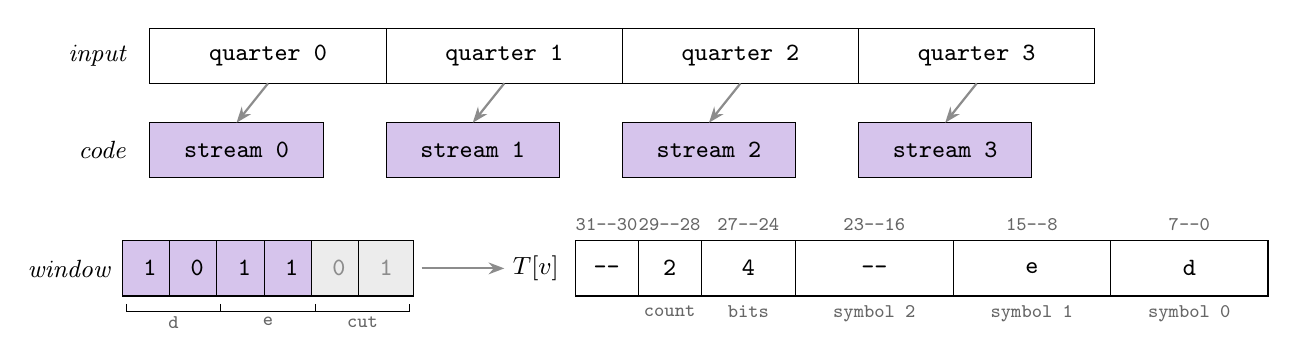
\begin{tikzpicture}[ads,bit/.style={cell,minimum width=6mm},
                       fld/.style={cell,minimum height=7mm}]
  % the input in quarters, each coded into its stream
  \node[var,anchor=east] at (-3mm,0) {input};
  \foreach \k in {0,1,2,3}
    {\node[cell,minimum width=30mm] (q-\k) at (15mm+\k*30mm,0)
       {quarter \k};
     \node[touched,minimum width=22mm] (st-\k) at (11mm+\k*30mm,-12mm)
       {stream \k};
     \draw[ptr,black!45] (q-\k.south) -- (st-\k.north);}
  \node[var,anchor=east] at (-3mm,-12mm) {code};
  % a window of W = 6 bits of a stream, in the order of reading
  \node[var,anchor=east] at (-5mm,-27mm) {window};
  \foreach \v/\s [count=\i from 0] in {1/touched,0/touched,1/touched,
                                       1/touched,0/free,1/free}
    \node[bit,\s] (w-\i) at (\i*6mm,-27mm) {\v};
  \foreach \a/\e/\t in {0/1/d,2/3/e,4/5/{cut}}
    \draw ($(w-\a.south west)+(0.5mm,-1mm)$) -- ++(0,-1mm)
          -| node[index,pos=0.25,below=0.6mm] {\t}
          ($(w-\e.south east)+(-0.5mm,-1mm)$);
  % the entry of the table for the window
  \node[var,anchor=east] (tv) at (52mm,-27mm) {$T[ v ]$};
  \foreach \t/\w/\x [count=\i from 0] in {{--}/8/0,{2}/8/8,{4}/12/16,
                                          {--}/20/28,{e}/20/48,{d}/20/68}
    \node[fld,minimum width=\w mm,anchor=west] (e-\i) at (54mm+\x mm,-27mm)
      {\t};
  \foreach \i/\t in {0/{31--30},1/{29--28},2/{27--24},3/{23--16},
                     4/{15--8},5/{7--0}}
    \node[index,above=1.2mm of e-\i] {\t};
  \foreach \i/\t in {1/count,2/bits,3/symbol 2,4/symbol 1,5/symbol 0}
    \node[index,below=1.2mm of e-\i] {\t};
  \draw[ptr,black!45] ($(w-5.east)+(1mm,0)$) -- ($(tv.west)+(-1mm,0)$);
\end{tikzpicture}
\end{document}
